\section{Pattern Language}

This section describes subset of PltRedex's pattern specification language supported by \texttt{PyPltRedex}. Grammar for the pattern language can be seen below, in EBNF notation. 

\begin{lstlisting}
pattern = number 
        | integer 
		| real 
		| natural 
		| string 
		| boolean 
		| variable-not-otherwise-mentioned 
		| hole 
		| symbol
        | (in-hole pattern pattern)
        | (pattern-sequence *) 
pattern-sequence : pattern 
                 | pattern ...  # literal ellipsis
\end{lstlisting}

\begin{itemize}
\item
\textit{number} pattern matches any number.

\item
\textit{integer} matches any exact integer. 

\item
\textit{real} matches any real number.

\item
\textit{natural} matches any natural number; that is any non-negative integer.

\item
\textit{string} matches any string.

\item
\textit{boolean} matches any boolean - \texttt{\#t} or \texttt{\#f}.
\item
\textit{variable-not-otherwise-mentioned} matches any symbol that is not used as a literal in language definition. For example, if language definition contains pattern \texttt{(+ number number)} \textit{variable-not-otherwise-mentioned} will not match symbol \texttt{+}.

\item
\textit{hole} matches \texttt{hole} term exactly.

\item
\textit{symbol} matches any symbol except if its value coincides with non-terminal symbol in language definition.
\end{itemize}

All pattern above except \textit{hole} can be suffixed with underscore and identifier (for example, \textit{number\_1}) to create binding to matched term.

\begin{itemize}
\item
\textit{(in-hole pattern pattern)} traverses the term trying to match the second pattern; upon successful match the term matching the second pattern is replaced with term `hole` and then the first pattern is matched. First pattern must match exactly one hole.

\item
\textit{pattern-sequence} pattern matches a term list, where each pattern-sequence element matches an element of the list. Each individual pattern within the sequence can be suffixed with \texttt{...} (literal ellipsis) and that will match zero or more terms matching the pattern.
\end{itemize}

If patterns in the pattern-sequence are suffixed with the same identifier (e.g. \texttt{(number\_1 number\_1)})), then the match is contrained to terms that are equal. That means term \texttt{(1 1)} matches the pattern but \texttt{(1 2)} does not. For patterns in \textit{define-language} constraint checking is not performed. PltRedex provides other constraint checks but they will not be considered.

\section{Compile-time Representation of Patterns}

Throughout the report the following notation will be used to represent actual Python classes used to implement the pattern language. Actual Python source code can be seen on page (TODO-appendix reference). 

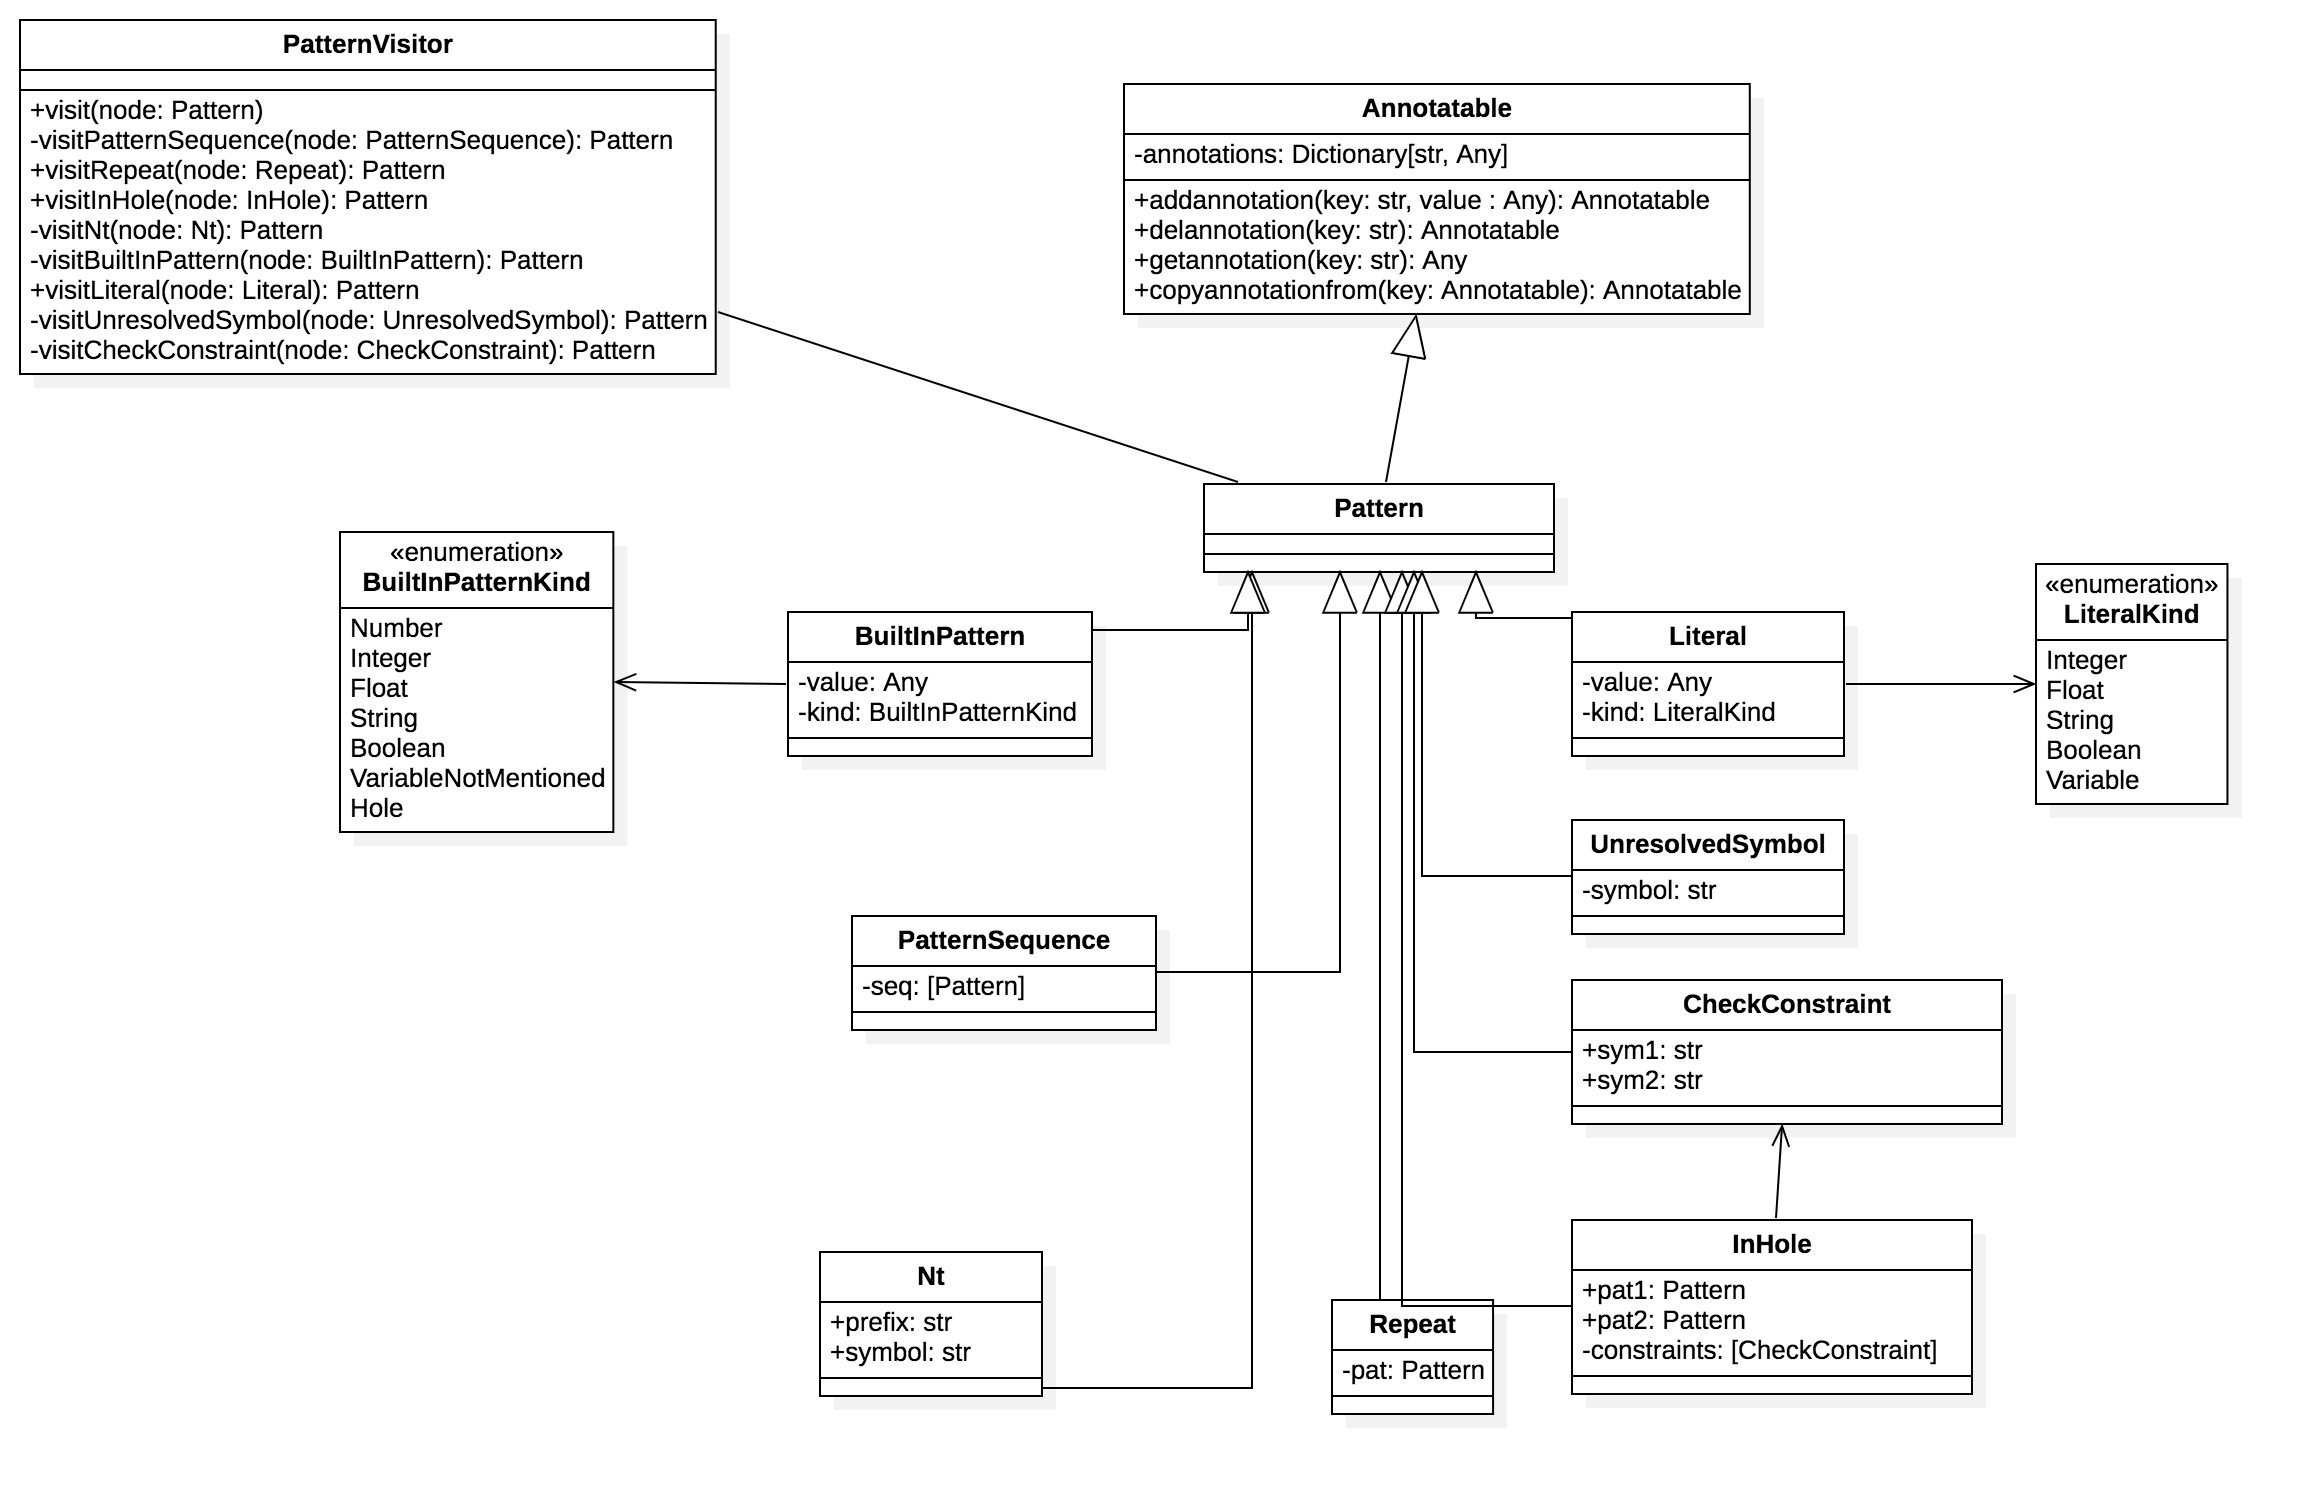
\includegraphics[scale=0.175]{class-diagram-pattern.png}


\begin{itemize}
\item
\PatternSequence represents `pattern-sequence` clause of the pattern language and may contain zero or more child patterns $p_i$.

\item 
\Repeat represents pattern $p$ under ellipsis.

\item 
\Nt represents non-terminal. $nt$ is a non-terminal symbol, while $s$ is the symbol used for binding terms. For example, given pattern \texttt{e\_1} $s$ is \texttt{e\_1} and $nt$ is \texttt{e}.
\item
\BuiltInPattern represents various built-in patterns such as \texttt{number} or \texttt{string}. $t$ is the tag and must be picked from set $T$. $s$ is the symbol used for binding terms.

\item
\InHolePattern represents \texttt{in-hole} pattern, $p_1$ and $p_2$ must be patterns.

\item 
\LiteralPattern represents a literal values in patterns. Since literal values can be of many types, a tag $l$ must be provided from set $T$. $v$ is actual literal value.

\item 
\UnresolvedSymbol used to represent symbols that are initially unknown to be non-terminal or literal, $s$ is the symbol.

\item
\CheckConstraint is used for equality checking of terms. Terms bound to $s_1$ and $s_2$ are checked for equality.

\end{itemize}

